\section{XSLT}

\begin{frame}
\frametitle{Transformación automática}
\begin{itemize}
\item	XSLT es otra propuesta del W3C. Es un lenguage para
	representar transformaciones de XML a otros lenguajes
	(incluído XML).
	\pause

\item	Definiendo las reglas podemos lograr algo que transforme
	de datos XML a, por ejemplo, una página web que los muestre.
\end{itemize}
\end{frame}

\begin{frame}
\centering
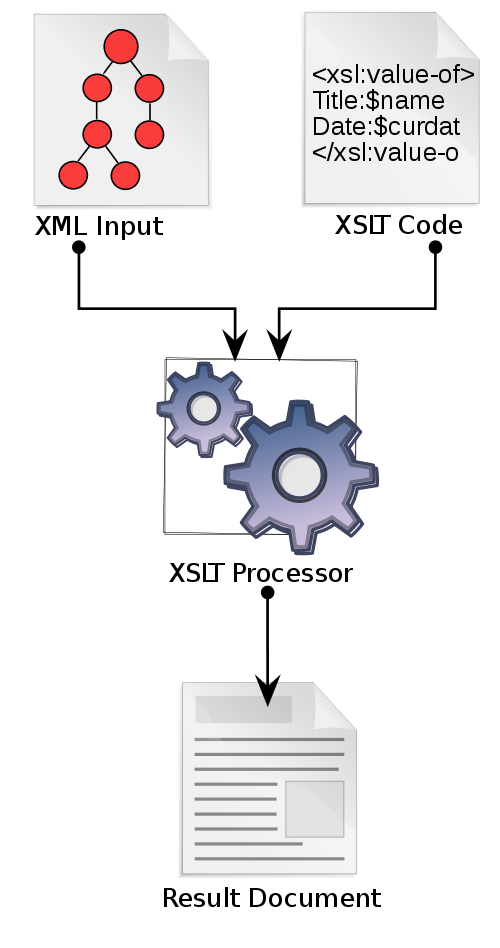
\includegraphics[scale=0.25]{xslt}
\end{frame}

\begin{frame}
\frametitle{Ejemplo - Documento original}

\footnotesize
\texttt{<persons>					\\
	~~<person username='JS1'>			\\
	~~~~<name>John</name>				\\
	~~~~<family-name>Smith</family-name>		\\
	~~</person>					\\
	~~<person username='MI1'>			\\
	~~~~<name>Morka</name>				\\
	~~~~<family-name>Ismincius</family-name>	\\
	~~</person>					\\
	</persons>}
\end{frame}
\begin{frame}
\frametitle{Ejemplo - Código XSLT}

\footnotesize
\texttt{<xsl:stylesheet version='1.0'>			\\
	~~<xsl:output method='xml' indent='yes'/>	\\
	~						\\
	~~<xsl:template match='/persons'>		\\
	~~~~<root>					\\
	~~~~~~<xsl:apply-templates select='person'/>	\\
	~~~~</root>					\\
	~~</xsl:template>				\\
	~						\\
	~~<xsl:template match='person'>			\\
	~~~~<name username='{@username}'>		\\
	~~~~~~<xsl:value-of select='name' />		\\
	~~~~</name>					\\
	~~</xsl:template>				\\
	</xsl:stylesheet>
	}
\end{frame}

\begin{frame}
\frametitle{Ejemplo - Resultado}

\footnotesize
\texttt{<root>						\\
	~~<name username='JS1'>John</name>		\\
	~~<name username='MI1'>Morka</name>		\\
	</root>
}
\end{frame}
